\documentclass[]{report}
\usepackage{graphicx}


% Title Page
\title{Report on state of the art}
\author{Developing 3D molecular representation}


\begin{document}
\maketitle
\section{New Reports}



\section{3D Molecular Representations Based on the Wave Transform for Convolutional Neural Networks $^{39}$}
Kuzminykh, Denis \& Polykovskiy, Daniil \& Kadurin, Artur \& Zhebrak, Alexander \& Baskov, Ivan \& Nikolenko, Sergey \& Shayakhmetov, Rim \& Zhavoronkov, Alexander. (2018). 3D Molecular Representations Based on the Wave Transform for Convolutional Neural Networks. Molecular Pharmaceutics.10.1021/acs.molpharmaceut.7b01134. 
\begin{enumerate}
	\subsection{Introduction}
	\item This work suggests using an autoencoder for developing conformations of molecules.
	\item A comparison between a previous and new approach is presented. New method is based on wave transform and the old one is voxel based representation.
	\subsection{Methodology}
	\item To represent a molecule in 3D. This work proposes to take PCA, to get the primary axes of molecules but not for dimentionality reduction. 
	\item \textbf{PCA} is a technique used for feature extraction and dimentionality reduction. It tries to identify the direction of maximum variance and project it to a new space with fewer or same dimensions. [1]
	\item Then translate the molecule in origin and orient it along the extracted reduction. 
	\item Discretize 3D space into a grid. Two atoms should not fall into the same 3D cell.
	\item Represent atoms in one-hot representation. Each voxel of the grid is represented as a binary vector that has at most one non-zero entry.
	\item Data set contained 9 most common atoms: H, C, N, O, F, S, Cl, Br, and I so the vector was a 9-D.
	\item This approach had two problems. One it could not capture the interaction of atoms. Second extreme sparcity. Less than 0.1\% voxels contain nonzero vectors.
	\item For solving these problems first \textbf{Gaussian smoothing} was used then \textbf{Smoothing with the Wave Transform}
	\item They convolve the  image with a Gaussian kernel. It removes sparsity , blurs the image and improves the results of a CNN.
	\item Wave transform method uses the idea of replacing atoms with circular waves emitting from it. Same convolution operation was used in it as well but with a different kernel.
	\item This performs better as it reduces sparsity more than Gaussian method and it removes its deficits. This representation can be used to extract chemical properties.
	\subsection{Conclusion}
	\item Experiments were performed on Zinc database, consisting of 4.5 million molecules with 3D coordinates.
	\item Wave based smoothing performs better results when it comes to redundancy, and independence problems.
\end{enumerate}

\section{Molecular Representation Going Long on Fingerprints$^{14}$}
Lagnajit Pattanaik, Connor W. Coley,
Molecular Representation: Going Long on Fingerprints,
Chem,
Volume 6, Issue 6,
2020,
Pages 1204-1207,
ISSN 2451-9294,
https://doi.org/10.1016/j.chempr.2020.05.002.

\begin{enumerate}
	\item This paper presents a basic understanding and overview of the different approaches or Ml models that can be used for representing molecular structures.
	\item It concatenates fingerprints into a multiple fingerprint feature. Combines it with a simple machine learning approach called random forest.
	\item It does not emphasize on 3D.
\end{enumerate}

\section{3DMol-Net: Learn 3D Molecular Representation using Adaptive Graph Convolutional Network Based on Rotation Invariance$^{2}$}
C. Li, W. Wei, J. Li, J. Yao, X. Zeng and Z. Lv, "3DMol-Net: Learn 3D Molecular Representation using Adaptive Graph Convolutional Network Based on Rotation Invariance," in IEEE Journal of Biomedical and Health Informatics, doi: 10.1109/JBHI.2021.3089162.
\begin{enumerate}
	\subsection{Introduction}
	\item This paper presents a 3D model called 3DMol-Net. It uses graph convolutional neural network to predict certain chemical properties and biochemical activities of molecules
	\item The methods for molecular 3D representation have run into limits, such as a huge number of parameters and memory requirements.
	\subsection{Methodology}
	\item It is based \textbf{rotation Invariance (RI)}. It is an adaptive graph convolutional model which can extract the relationships among nodes and then make a 3D graph Laplacian.
	\item Laplacian is a way to represent graphs in matrix forms and these matrices can give us a lot of information about graphs.
	\item Rotation Invariance Mapping (RIM) is used for learning the 3D features of molecules that are 3D graph Laplacian.
	\item If arbitrary rotations are applied on a function and it's values do not change then it is said to have rotation invariance.[2]
	\item The classic CNN is capable of learning RI with data augementatio(rotation, scaling etc).
	\item This model focuses to 3D structure and RI to get the representation of molecules. It has 2 parts: (i) 3D graph Laplacian
	with soft relations (ii) rotation-invariant mapping.
	
	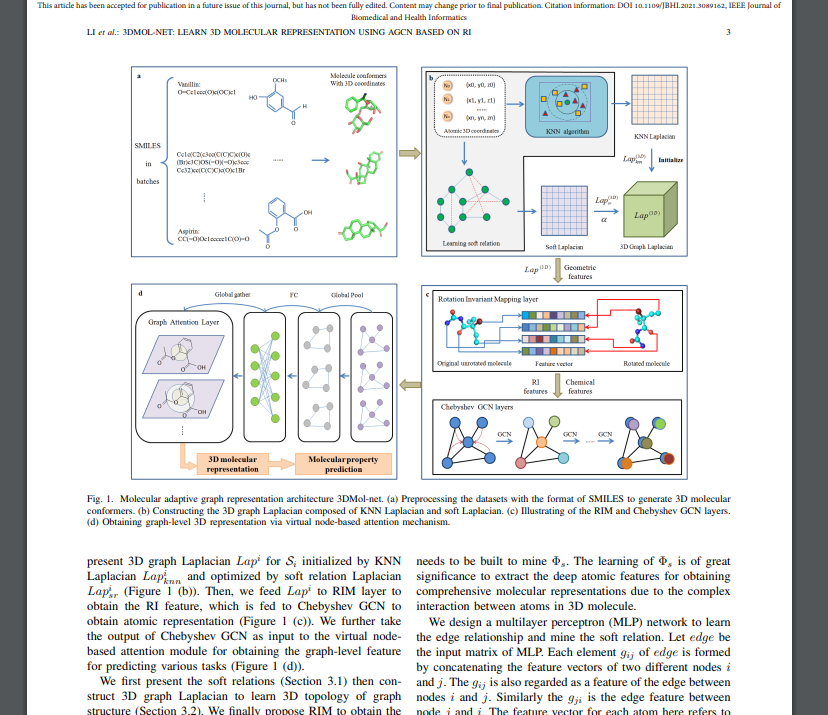
\includegraphics[width=\linewidth]{3DMol-net}
	\item  Chebyshev GCN is for prediction of molecular properties
	\subsection{Conclusion}
	\item In comparison with other state of the art methods, this model showed good results.
\end{enumerate}

\section{Highly accurate protein structure prediction with AlphaFold}
umper, J., Evans, R., Pritzel, A. et al. Highly accurate protein structure prediction with AlphaFold. Nature 596, 583–589 (2021). https://doi.org/10.1038/s41586-021-03819-2
	\subsection{Introduction}
	\begin{enumerate}
	\item This paper uses AlphaFold to buid a model that can predict the structure of a molecule.
	\item In difficult scenarios like entangled homomers or proteins, AlphaFold can handle missing physical background and build reliable models.
	\item All 3D coordinates are directly predicted by the AlphaFold network.
	\subsection{Methodology}
	\item 	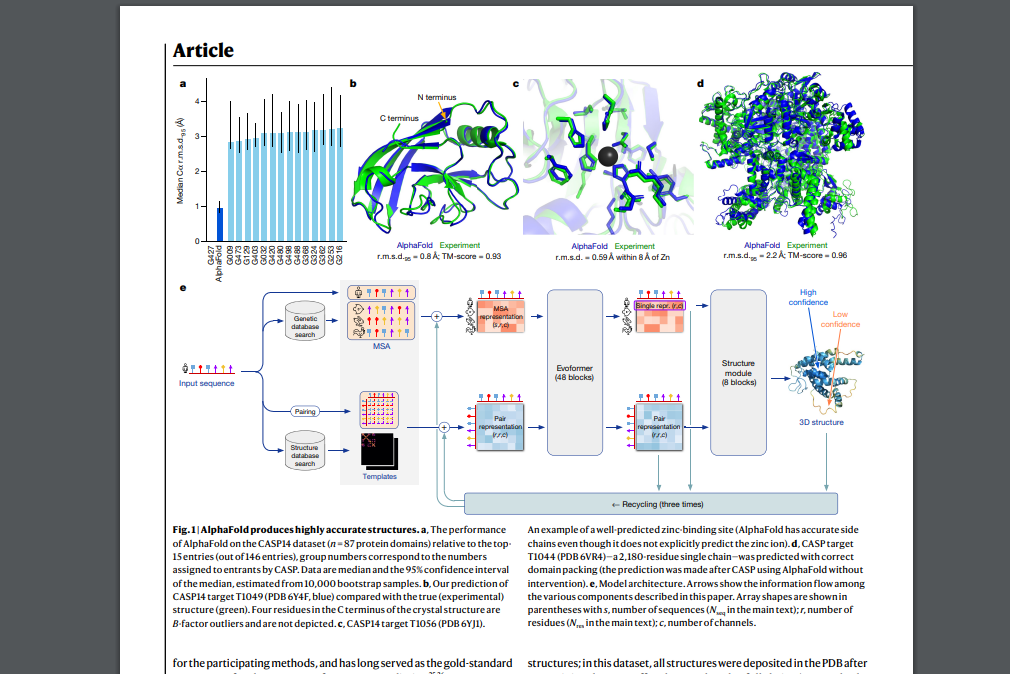
\includegraphics[width=\linewidth]{AlphaFold}
	\end{enumerate}
\section{CONFORMATION-GUIDED MOLECULAR REPRESENTATION WITH HAMILTONIAN NEURAL NETWORKS$^{3}$}
Li, Ziyao \& Yang, Shuwen \& Song, Guojie \& Cai, Lingsheng. (2021). Conformation-Guided Molecular Representation with Hamiltonian Neural Networks. 
\begin{enumerate}
	\subsection{Introduction}
	\item Molecular Hamiltonian Network, a unique molecular representation technique, is proposed in this research.
	\item Hamiltonian Engine (HE) and the Fingerprint Generator are the two primary components of the module (FG).
	\item GNN+LSTM is used to produce locations and momentum from an input which is a molecular graph with atom and bond data.
	\item These ps and qs are fed into a Hamiltonian system, which generates "molecular configurations."
	\item A message passing algorithm is used as well.
	\subsection{Conclusion}
	\item In the experiments QM9 was used.
	\item The model was able to learn the conformers and presented state of the art performance in property prediction.
\end{enumerate}
\section{Pushing the Boundaries of Molecular Representation for Drug Discovery with the Graph Attention Mechanism $^{88}$}
Xiong, Zhaoping \& Wang, Dingyan \& Liu, Xiaohong \& Feisheng, Zhong \& Wan, Xiaozhe \& Li, Xutong \& Li, Zhaojun \& Luo, Xiaomin \& Chen, Kaixian \& Jiang, H. \& Zheng, Mingyue. (2019). Pushing the boundaries of molecular representation for drug discovery with graph attention mechanism. Journal of Medicinal Chemistry. 63. 10.1021/acs.jmedchem.9b00959. 
\begin{enumerate}
	\subsection{Introduction}
	\item This work proposes Attentive FP, a new graph-based neural network architecture for representing molecules.
	\item Attentive FP is capable of efficiently capturing the hidden linkage between any nodes.
	\item The basic idea behind employing the attention mechanism on a graph is to get a context vector for the target node by focusing on its neighbors and immediate surroundings.
	\item Model can be divided into has 3 parts: (1) alignment, (2) weighting, and (3) context.
	\item 	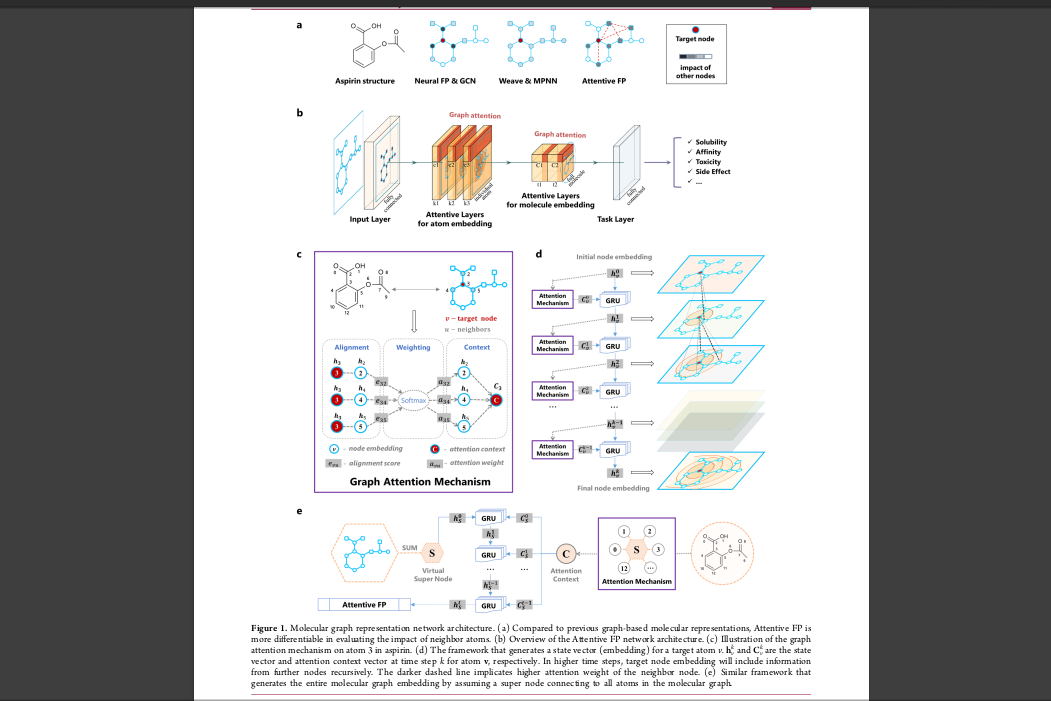
\includegraphics[width=\linewidth]{AttentiveFP}
	\subsection{Conclusion}
	\item To check the performance of Attentive FP, three different data sets were used and it performed very well.
\end{enumerate}
\section{TrimNet: learning molecular representation from triplet messages for biomedicine $4$}
Pengyong Li, Yuquan Li, Chang-Yu Hsieh, Shengyu Zhang, Xianggen Liu, Huanxiang Liu, Sen Song, Xiaojun Yao, TrimNet: learning molecular representation from triplet messages for biomedicine, Briefings in Bioinformatics, Volume 22, Issue 4, July 2021, bbaa266, https://doi.org/10.1093/bib/bbaa266
\begin{enumerate}
\subsection{Introduction}
	\item The aim of this paper is to devise a new method using triplet message
	mechanism to learn molecular representations. This graph based ap-
	proach has been named as TrimNet.
	\item Model presented in this paper has a message phase and a readout phase.
	\item Many datasets like QM9, MUV, HIV, BACE, Tox21, ToxCast, SIDER,
	ClinTox, Human and C.elegan have been used in this work. The
	data set was balanced with negative and positive samples.
	\subsection{Methodology}
	\item A triplet edge network was used for reducing the computational
	cost and increase the performance. This network collects the infor-
	mation from the neighbours as well.
	\item For training the model batch gradient descent and error back-
	propagation algorithms were used. To avoid over fitting of the
	model, dropout and weight decay were the methods implemented
	for regularization.
	\item PyTorch was used for the model. V100 and TITAN Black graphic
	cards were used for the training and testing purposes.
	\item In the model a graph structure is used for the representation of
	features. This model achieved state-of-the-art performance for six
	out of eight data sets in testing.
	\item Prediction of CPI is an important feature and the model was eval-
	uated while using a previous approach and after comparison this
	model showed improved results.
	\subsection{Conclusion}
	\item QM9 dataset was used for experimentation.
	\item TrimNet showed remarkable results for molecular representations
	another amazing feature of TrimNet includes lessened number of
	parameters.
\end{enumerate}
\section{Structure/Response Correlations and Similarity/Diversity Analysis by GETAWAY Descriptors, 2. Application of the Novel 3D Molecular Descriptors to QSAR/QSPR Studies$ ^{462}$}

\begin{enumerate}
	\item Old paper. It presents an approach that is not using Ml. In this work molecular representation that can be simply calculated using the spatial coordinates of the molecule atoms in a specific conformation.
\end{enumerate}


\section{New Reports based}
\begin{enumerate}
	\item 
\end{enumerate}
\section{title}
\begin{enumerate}
	\item 
\end{enumerate}
\section{title}
\begin{enumerate}
	\item 
\end{enumerate}
\section{title}
\begin{enumerate}
	\item 
\end{enumerate}

\section{title}
\begin{enumerate}
	\item 
\end{enumerate}
\section{title}
\begin{enumerate}
	\item 
\end{enumerate}


\section{Refrences}
1. https://vitalflux.com/feature-extraction-pca-python-example/
2. https://en.wikipedia.org/wiki/Rotational\_invariance 

\end{document}          
